%%%%%%%%%%%%%%%%%%%%%%%%%%%%%%%%%%%%%%%%%%%%%%%%%%%%%%%%
%%%%%%%%%%%%%%%%%%%%%%%%%%%%%%%%%%%%%%%%%%%%%%%%%%%%%%%%
\section{Materials and Methods}
%%%%%%%%%%%%%%%%%%%%%%%%%%%%%%%%%%%%%%%%%%%%%%%%%%%%%%%%
%%%%%%%%%%%%%%%%%%%%%%%%%%%%%%%%%%%%%%%%%%%%%%%%%%%%%%%%

FIM 3 is a fully operational pipeline of software tools to help acquire datasets, cache hydrofabrics, produce FIMs, and evaluate results.

%%%%%%%%%%%%%%%%%%%%%%%%%%%%%%%%%%%%%%%%%%%%%%%%%%%%%%%%
\subsection{Software Architecture and Dependencies}
%%%%%%%%%%%%%%%%%%%%%%%%%%%%%%%%%%%%%%%%%%%%%%%%%%%%%%%%

FIM 3 exclusively uses free and open source software dependencies (FOSS) and only depends on a host machine having Docker installed on it. 
Within a customized Docker image, a series of dependencies are employed including but not limited to Python 3, GDAL, TauDEM, RichDEM, and Geographic Resource Analysis Support System (GRASS).

%%%%%%%%%%%%%%%%%%%%%%%%%%%%%%%%%%%%%%%%%%%%%%%%%%%%%%%%
\subsection{Datasets}
%%%%%%%%%%%%%%%%%%%%%%%%%%%%%%%%%%%%%%%%%%%%%%%%%%%%%%%%

All data sources used within FIM 3 are publicly available from a variety of government sources including the USGS, NWC, Federal Emergency Management Agency (FEMA), and US Army Core of Engineers (USACE) to enhance reproducibility and collaboration among government, academia, and industry.
The National Hydrography Dataset Plus High Resolution (NHDPlusHR) Beta Version is the latest hydrography dataset used for land surface hydrologic modeling in the US \cite{moore2019user}. 
It is used in conjunction with the hydrofabric of the NWM V2.1 to help define flowlines for FIM 3 while the NWM hydrofabric is also used to define reservoirs for exclusion and catchments to cross-walk to for forecasting purposes.
The AHPS forecast points are required to determine the RnR downstream segments in order to define the RnR Mainstems (MS).
For enforcing levee data into the NED DEMs, the USACE National Levee Database (NLD) is used via burning feature elevations \cite{engineers2016national}.
Additionally, FEMA Base Level Engineering (BLE) from Region 6 (parts of Texas, Oklahoma, Arkansas, Louisiana and New Mexico) 1\% (100 year) and 0.2\% (500 year) datasets are used as validation in this study. 
These BLE datasets are provided at the watershed scale (HUC8) utilizing best available simulations and DEMs.
The full input datasets sorted by source are listed below:

\begin{enumerate}
\item{USGS - NHDPlusHR Beta}
    \begin{enumerate}
    \item{\textit{BurnLineEvents:} flowlines used by NHDPlusHR for hydro-enforcing DEM}
    \item{\textit{Value-Added Attributes:} database of additional attributes referenced to flowlines that enhance navigation, analysis, and display}
    \item{\textit{DEM:} DEM from National Elevation Dataset (NED) in 10m (or 1/3 arc-second) spatial resolution with vertical units in centimeters \cite{gesch2002national}}
    \end{enumerate}
\item{NOAA OWP - NWM V2.1 Hydrofabric}
    \begin{enumerate}
    \item{\textit{flowlines:} stream network center lines used for NWM routing and forecasting}
    \item{\textit{reach level catchments:} surface drainage area corresponding to each river reach}
    \item{\textit{waterbodies:} includes reservoirs, lakes, and others that are modeled within the NWM}
    \end{enumerate}
\item{NOAA OWP - AHPS Forecast Points}
    \begin{enumerate}
    \item{\textit{AHPS:} Collection AHPS forecast points to associate to RnR Mainstems}
    \end{enumerate}
\item{USACE - NLD}
    \begin{enumerate}
    \item{\textit{Levee elevations:} Top of levee elevations are gathered with in the NLD provided by USACE for hydro-enforcement}
    \end{enumerate}
\item{FEMA BLE}
    \begin{enumerate}
    \item{\textit{cross-sections:} cross-sections and associated data for associating 1\% and 0.2\% recurrence discharges with NWM reaches}
    \item{\textit{flood inundation maps:} FIMs produced by BLE at the two recurrence intervals for comparison with FIMs from OWP FIM versions}
    \end{enumerate}
\end{enumerate}

%%%%%%%%%%%%%%%%%%%%%%%%%%%%%%%%%%%%%%%%%%%%%%%%%%%%%%%%
\subsection{Hydro-conditioning}
%%%%%%%%%%%%%%%%%%%%%%%%%%%%%%%%%%%%%%%%%%%%%%%%%%%%%%%%

The DEM from the NED is subject to a series of hydro-conditioning procedures to enhance it's suitability for riverine flood inundation mapping. 
These techniques are specific for making FIM and different than the conditioning methods used by the NHDPlusHR Beta \cite{moore2019user}.
Hydro-conditioning is implemented to obtain many objectives including enforcing the location of hydrologically relevant features such as flowlines, lakes, or drainage divides whether natural or anthropogenic. 
It can also be used to simulate more accurate bathymetry which is not accounted for in the NED 10m DEM \cite{gesch2002national}.

Specifically within the context of FIM 3, the hydro-conditioning operations that take place in sequential order are presented.
Prior to any hydro-conditioning, all input datasets must be subset from their original spatial domain scales into the processing unit designated at run time which can be either HUC 4, 6 or 8. 
The subsetting is done by spatial query for the cases of the levees, DEM, and NWM hydrofabric while the NHDPlusHR BurnLineEvents are subset via attribute query for the given reachcode's membership in the processing unit.

%%%%%%%%%%%%%%%%%%%%%%%%%%%%%%%%%%%%%%%%%%%%%%%%%%%%%%%%
\subsubsection{Headwater Seed Points} 

The locations used for seeding headwater locations were enforced to provide identical stream density as the NWM V2.1 Flowlines while utilizing the exact locations of streams found in the NHDPlusHR Beta that have much higher stream densities. 
This was accomplished by finding the NHDPlusHR headwater most adjacent to every NWM headwater point. 
This point is later used for initializing the construction of a FIM 3 specific flowline network that agrees with its resulting flow directions.

%%%%%%%%%%%%%%%%%%%%%%%%%%%%%%%%%%%%%%%%%%%%%%%%%%%%%%%%
\subsubsection{Stream locations and Bathymetry}

The subset of the NHDPlusHR Beta headwater seed points used in this study are then employed in deriving the remaining stream network used for enforcing the stream network and its associated bathymetry. 
All NHDPlusHR Beta BurnLineEvents downstream of the subset headwater points are selected for hydro-enforcement. 
This results in a stream network that has the same density as the NWM V2.1 flowline network but utilizes the locations of the NHDPlusHR Beta BurnLineEvents. 

\note[Fernando Aristizabal]{For Trevor Grout}
This trimmed stream network is then utilized to hydro-enforce the DEM with a methodology developed by \citeA{hellweger1997agree} known as AGREE DEM Surface Reconditioning System. 
The AGREE algorithm seeks to burn artificially deep thalweg elevations by a uniform value known as sharp drop. 
The modification continues by excavating an area of a given buffer distance from the thalweg by a depth proportional to the distance from the channel given by the smooth drop. 
The resulting enforcement of the thalweg and general bathymetric region results in a cross-section resembling a trapezoidal shape with a significantly lower elevation along the thalweg line only as can be seen in \ref{fig:agree_dem_cross_section}.
In total, the AGREE algorithm requires three parameters including the buffer distance, smooth drop, and sharp drop. 
Using simple thalweg burning techniques as opposed to the full AGREE method helps prevent distortions in the delineation of streams as well as the catchment boundaries \cite{saunders1995grid,saunders1996gis,mizgalewicz1996modeling,hellweger1997agree,quenzer1998gis,baker2006comparison,}.
\citeA{baker2006comparison} noted AGREE produced satisfactory results when compared to other enforcement especially when computational costs are considered. 
Downsides to the technique include the possibility of exhibiting parallel streams where the burned stream and real stream are both represented \cite{hellweger1997agree,saunders1999preparation} and some distortion of the catchment boundaries can also be observed \cite{saunders1999preparation,saunders1996gis}. Some of these drawbacks are later addressed by additional conditioning techniques later on.

\begin{figure}[h!]
\centering
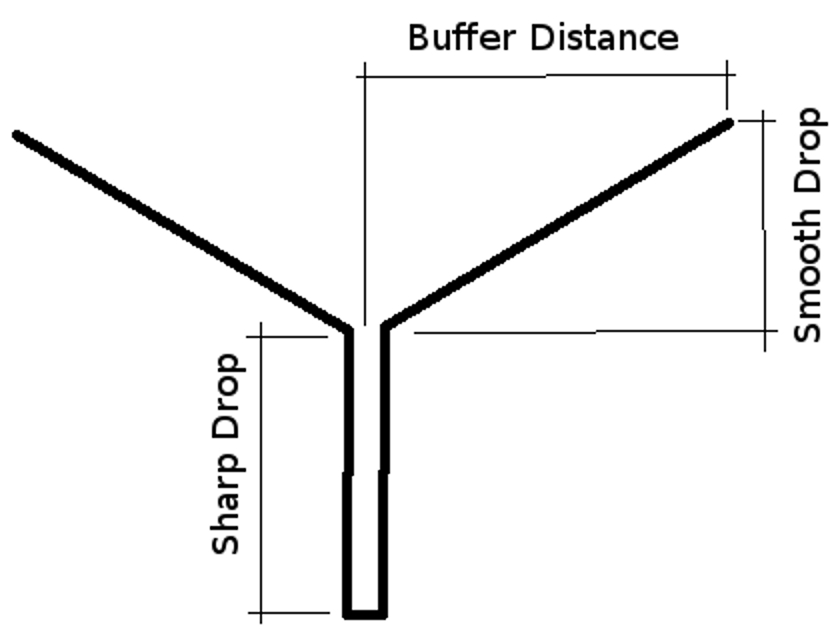
\includegraphics[scale=1.0]{figures/agree_dem_cross_section.jpg}
\caption{Placeholder for figure demonstrating AGREE method}
\label{fig:agree_dem_cross_section}
\end{figure}


%%%%%%%%%%%%%%%%%%%%%%%%%%%%%%%%%%%%%%%%%%%%%%%%%%%%%%%%
\subsubsection{Levee Data}

\note[Fernando Aristizabal]{For Ryan Spies}
Levee data from the NLD was compiled and projected in order to enforce levee elevations within the NED 10m DEM.

%%%%%%%%%%%%%%%%%%%%%%%%%%%%%%%%%%%%%%%%%%%%%%%%%%%%%%%%
\subsubsection{Pit Removal}
\cite{barnes2014efficient}

%%%%%%%%%%%%%%%%%%%%%%%%%%%%%%%%%%%%%%%%%%%%%%%%%%%%%%%%
\subsubsection{Stream Thalweg Elevation Conditioning}

In order to prevent parallel streams where the steep burned streams and the original streams occur, the normalized excavation algorithm \cite{saunders1999preparation} is used to seek a zonal (nearest neighbor) elevation minimum for each thalweg pixel. 
Each zone is defined as the thalweg's pixel nearest neighborhood within a maximum distance of 50m.

%%%%%%%%%%%%%%%%%%%%%%%%%%%%%%%%%%%%%%%%%%%%%%%%%%%%%%%%
\subsection{Deriving FIM Hydrofabric}
%%%%%%%%%%%%%%%%%%%%%%%%%%%%%%%%%%%%%%%%%%%%%%%%%%%%%%%%

%%%%%%%%%%%%%%%%%%%%%%%%%%%%%%%%%%%%%%%%%%%%%%%%%%%%%%%%
\subsubsection{Flow directions and Flat Resolution}
\cite{survila2016scalable,tarboton1997new,wallis2009parallel}

%%%%%%%%%%%%%%%%%%%%%%%%%%%%%%%%%%%%%%%%%%%%%%%%%%%%%%%%
\subsubsection{Stream Network}
\cite{wallis2009parallel}

%%%%%%%%%%%%%%%%%%%%%%%%%%%%%%%%%%%%%%%%%%%%%%%%%%%%%%%%
\subsubsection{Reach Catchments}

%%%%%%%%%%%%%%%%%%%%%%%%%%%%%%%%%%%%%%%%%%%%%%%%%%%%%%%%
\subsubsection{HAND}

%%%%%%%%%%%%%%%%%%%%%%%%%%%%%%%%%%%%%%%%%%%%%%%%%%%%%%%%
\subsubsection{Synthetic Rating Curves}

%%%%%%%%%%%%%%%%%%%%%%%%%%%%%%%%%%%%%%%%%%%%%%%%%%%%%%%%
\subsection{RnR Mainstems Method}
%%%%%%%%%%%%%%%%%%%%%%%%%%%%%%%%%%%%%%%%%%%%%%%%%%%%%%%%

%%%%%%%%%%%%%%%%%%%%%%%%%%%%%%%%%%%%%%%%%%%%%%%%%%%%%%%%
\subsection{Evaluation and Testing}
%%%%%%%%%%%%%%%%%%%%%%%%%%%%%%%%%%%%%%%%%%%%%%%%%%%%%%%%

